%% 10. Parallel Primitives

% Reductions

\begin{frame}{Parallel Primitives}

\begin{block}{Reductions}
  \begin{itemize}
   \item Use $N$ values to compute $1$ result value
   \item Examples: Dot-products, vector norms, etc.
  \end{itemize}
\end{block}

\begin{block}{Reductions with Few Threads}
  \begin{itemize}
   \item Decompose $N$ into chunks for each thread
   \item Compute chunks in parallel
   \item Merge results with single thread
  \end{itemize}
\end{block}

\begin{center} 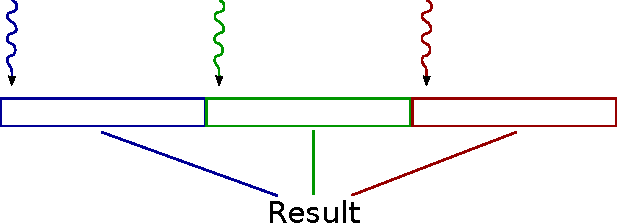
\includegraphics[width=0.7\textwidth]{figures/reductions-thread} \end{center}

\end{frame}





\begin{frame}{Parallel Primitives}

\begin{block}{Reductions with Many Threads}
  \begin{itemize}
   \item Decompose $N$ into chunks for each workgroup
   \item Use fast on-chip synchronization within each workgroup
   \item Sum result for each workgroup separately
  \end{itemize}
\end{block}

\begin{center} 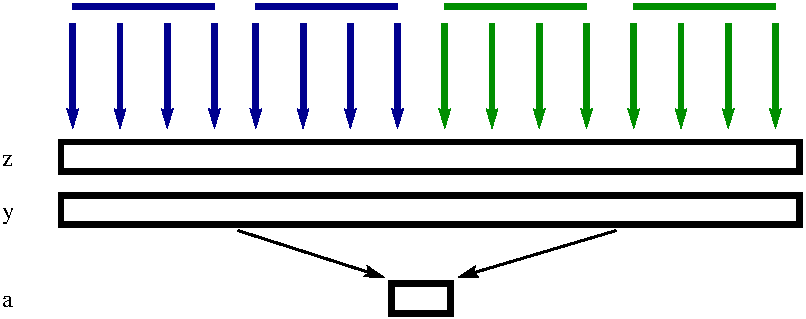
\includegraphics[width=0.8\textwidth]{figures/inner-product-kernel} \end{center}


\end{frame}


%%

\begin{frame}[fragile]{Parallel Primitives}

\begin{block}{Reductions with Many Threads}
  \vspace*{-.2cm}
\begin{center} 
  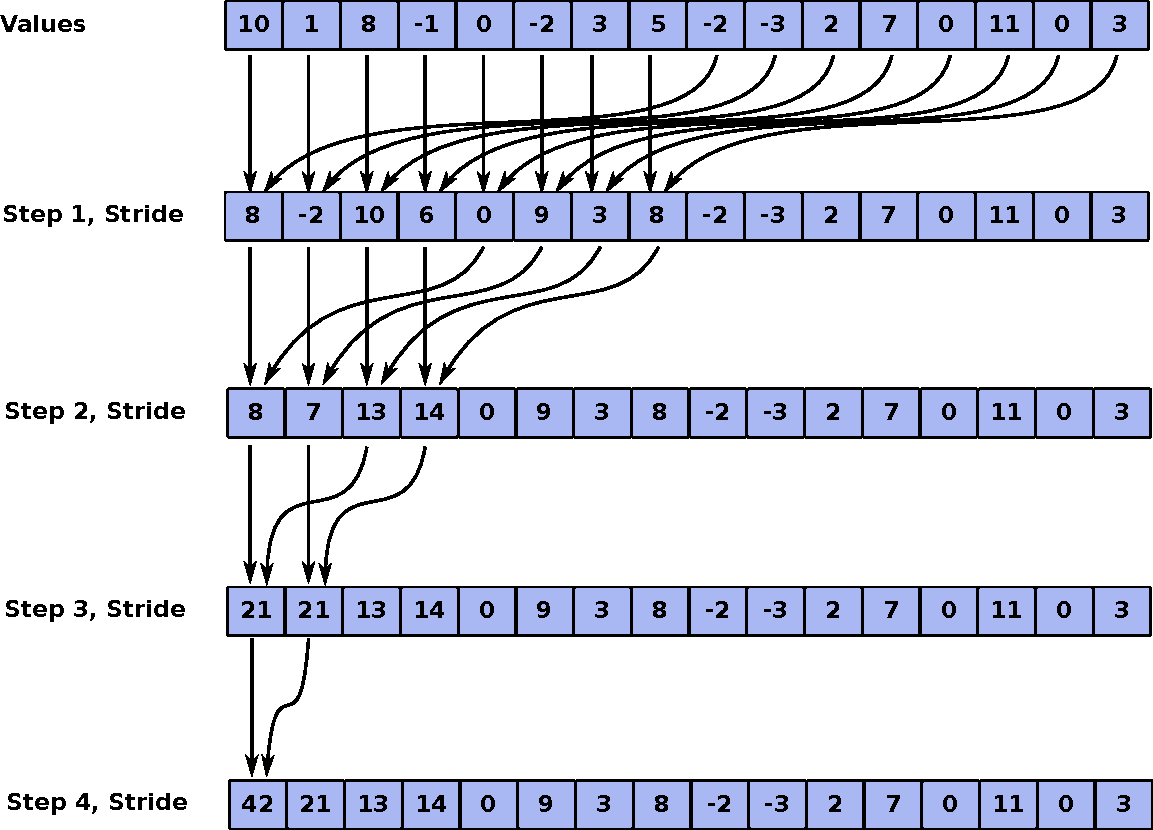
\includegraphics[width=0.6\textwidth]{figures/reduction}
\end{center}
\end{block}
  \vspace*{-.5cm}
\begin{center}
\begin{lstlisting}
shared_m[threadIdx.x] = thread_sum;
for (int stride = blockDim.x/2; stride>0; stride/=2) {
  __syncthreads();
  if (threadIdx.x < stride)
    shared_m[threadIdx.x] += shared_m[threadIdx.x+stride];
}
\end{lstlisting}
\end{center}

\end{frame}



%%%%%%%%%%%%% Load and FLOPs: Use shared memory





%%%%%%%%%%%% Prefix sum: Explain why and how it works. Use FEM as example

\begin{frame}[fragile]{Parallel Primitives}

\begin{minipage}{0.7\textwidth}
\begin{block}{Prefix Sum}
  \begin{itemize}
   \item Inclusive: Determine $y_i = \sum_{k=1}^i x_k$
   \item Exclusive: Determine $y_i = \sum_{k=1}^{i-1} x_k$, $y_1 = 0$
  \end{itemize}
\end{block}

%\pause
\begin{block}{Example}
 \begin{itemize}
  \item x: $4$, $3$,  $\hphantom{1}6$,  $\hphantom{1}5$,  $\hphantom{1}4$,  $\hphantom{1}7$,  $\hphantom{1}4$,  $\hphantom{1}4$,  $\hphantom{1}4$
  \item y: $4$, $7$,             $13$,             $18$,             $22$,             $29$,             $33$,             $37$,             $41$ (inclusive)
  \item y: $0$, $4$,  $\hphantom{1}7$,             $13$,             $18$,             $22$,             $29$,             $33$,             $37$ (exclusive)
 \end{itemize}

\end{block}

\begin{block}{Applications}
  \begin{itemize}
   \item Sparse matrix setup
   \item Graph algorithms
  \end{itemize}
\end{block}
\vspace*{1cm}
\end{minipage}
\begin{minipage}{0.2\textwidth}
\vspace*{4cm} \hspace*{-3.5cm}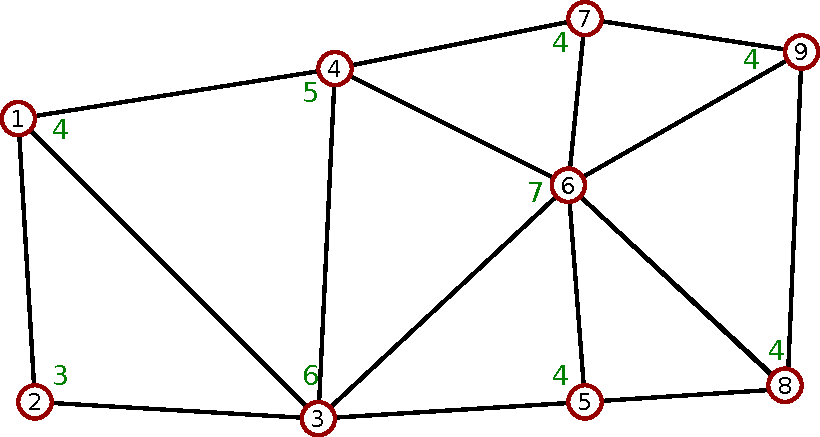
\includegraphics[width=2.8\textwidth]{figures/graph-1}
\end{minipage}

\end{frame}


%%


\begin{frame}[fragile]{Parallel Primitives}

 \begin{block}{Prefix Sum Implementation}
  \begin{center} 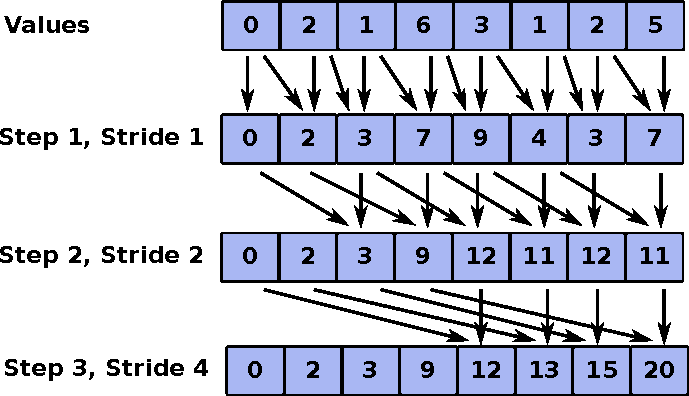
\includegraphics[width=0.5\textwidth]{figures/prefix-sum} \end{center}
  \begin{lstlisting}
for(int stride = 1; stride < blockDim.x; stride *= 2)
{
  __syncthreads();
  shared_buffer[threadIdx.x] = my_value;
  __syncthreads();
  if (threadIdx.x >= stride)
    my_value += shared_buffer[threadIdx.x - stride];
}
__syncthreads();
shared_buffer[threadIdx.x] = my_value;
  \end{lstlisting}
 \end{block}
\end{frame}


%%
%%%%%%%%%%%% Libraries
%%


\begin{frame}[fragile]
\frametitle{Parallel Primitives}

 \begin{block}{Other Parallel Primitives}
  \begin{itemize}
   \item Sort
   \item Gather and Scatter
   \item Load to shared memory and work there
   \item etc.
  \end{itemize}
 \end{block}

 \begin{block}{GPU-Accelerated Software Libraries}
  \begin{itemize}
   \item Linear Algebra: ViennaCL, MAGMA, CUSP, VexCL, ...
   \item Solvers: ViennaCL, MAGMA, cuSolver, Paralution, clAMG, ...
   \item FFT: cuFFT, clFFT, FFTW, ...
   \item Primitives: VexCL, Boost.Compute, ...
   \item Machine Learning: Caffe, cuDNN, ...
  \end{itemize}
 \end{block}

\end{frame}

